% Double-column laboratory report template
% Adapted from original laboratory report layouts by Karol Cieślik (2017–2018).
% The sample content and numerical values below are fictional.
% Compile with pdfLaTeX + BibTeX, or use latexmk -pdf.

\documentclass[10pt,a4paper]{article}

\usepackage[T1]{fontenc}
\usepackage[utf8]{inputenc}
\usepackage[english]{babel}
\usepackage{lmodern}
\usepackage[margin=1.8cm]{geometry}
\usepackage{microtype}
\usepackage{amsmath}
\usepackage{booktabs}
\usepackage{graphicx}
\usepackage{pgfplots}
\usepackage{natbib}
\usepackage{fancyhdr}
\usepackage{xcolor}
\usepackage{titlesec}
\usepackage{caption}
\usepackage[hidelinks]{hyperref}

\pgfplotsset{compat=1.18}
\definecolor{reportaccent}{HTML}{245473}
\definecolor{reportmuted}{HTML}{647483}
\colorlet{reportgrid}{black!12}
\titleformat{\section}{\normalfont\large\bfseries\color{reportaccent}}{\thesection}{0.7em}{}
\titlespacing*{\section}{0pt}{1.9ex plus 0.6ex minus 0.2ex}{0.7ex}
\captionsetup{font=small,labelfont={bf,color=reportaccent},skip=6pt}
\setlength{\columnsep}{0.8cm}
\setlength{\parindent}{0.4cm}
\setlength{\parskip}{0.1em}
\setlength{\headheight}{15pt}
\emergencystretch=1em

% -------------------- Edit these fields --------------------
\newcommand{\reporttitle}{Electrical Characterisation of a Resistor}
\newcommand{\reportshorttitle}{Laboratory Report}
\newcommand{\reportauthor}{Student Name}
\newcommand{\reportinstitution}{Institution or Laboratory Name}
\newcommand{\reportcourse}{Course or Research Group}
\newcommand{\reportsupervisor}{Supervisor Name}
\newcommand{\reportdate}{\today}
% -----------------------------------------------------------

\pagestyle{fancy}
\fancyhf{}
\fancyhead[L]{\small\color{reportmuted}\reportshorttitle}
\fancyhead[R]{\small\color{reportmuted}\reportauthor}
\fancyfoot[R]{\thepage}
\renewcommand{\headrulewidth}{0.3pt}

\begin{document}
% Avoid duplicate PDF page destinations when the page counter restarts
% after the unnumbered title page.
\hypersetup{pageanchor=false}
\begin{titlepage}
  \centering
  \vspace*{2cm}
  {\large\color{reportmuted}\scshape\reportinstitution\par}
  \vspace{0.35cm}
  {\normalsize\color{reportmuted}\reportcourse\par}
  \vspace{2.7cm}
  {\small\bfseries\color{reportaccent}\MakeUppercase{Laboratory Report}\par}
  \vspace{0.6cm}
  {\Huge\bfseries\reporttitle\par}
  \vspace{0.8cm}
  {\color{reportaccent}\rule{0.25\textwidth}{1.4pt}\par}
  \vfill
  {\large\bfseries\reportauthor\par}
  \vspace{0.35cm}
  {\normalsize\color{reportmuted}Supervisor: \reportsupervisor\par}
  \vspace{0.5cm}
  {\normalsize\reportdate\par}
  \vspace{1.0cm}
\end{titlepage}
\hypersetup{pageanchor=true}

% The title page is single-column; the body starts in two columns.
\twocolumn

\section*{Abstract}
This short example demonstrates a two-column scientific laboratory report.
An elementary resistor is the illustrative system. All reported measurements
and uncertainties are \textbf{synthetic}; no real experiment is described.
Replace this summary with the objective, method and actual main finding of
your laboratory work.

\section{Introduction}
\label{sec:introduction}
Explain the scientific question and the physical principles used to interpret
the experiment. For an ideal ohmic resistor, voltage \(V\) and current \(I\)
are related by
\begin{equation}
    V = IR,
    \label{eq:ohm}
\end{equation}
where \(R\) denotes resistance. Equation~\eqref{eq:ohm} shows an ordinary
numbered equation in a narrow column.

\section{Experimental Methods}
\label{sec:methods}
Describe the equipment, measurement sequence and uncertainties in sufficient
detail that another reader can understand the procedure. In this fictional
example, imagine a variable voltage source and a current meter connected to
a nominal \(1\,\mathrm{k}\Omega\) resistor.

Assume standard uncertainties of \(0.01\,\mathrm{V}\) and
\(0.03\,\mathrm{mA}\) for illustration. These values were not obtained by
calibration. The distinction between precision and accuracy, as well as
methods of uncertainty propagation, is discussed by \citet{taylor1997}.

\section{Results}
\label{sec:results}
Table~\ref{tab:data} illustrates numerical formatting. The values are
invented and should be replaced with genuine measurements before scientific
use. In a compact report, tables should be limited to quantities that
contribute directly to the argument.

\begin{table}[htbp]
    \centering
    \caption{Synthetic observations; not experimental data.}
    \label{tab:data}
    \begin{tabular}{@{}rr@{}}
        \toprule
        \(V\) (\(\mathrm{V}\)) & \(I\) (\(\mathrm{mA}\)) \\
        \midrule
        0.50 & 0.50 \\
        1.00 & 1.01 \\
        1.50 & 1.49 \\
        2.00 & 2.02 \\
        2.50 & 2.49 \\
        3.00 & 3.01 \\
        \bottomrule
    \end{tabular}
\end{table}

Figure~\ref{fig:current-voltage} is generated directly in LaTeX and fits
the width of one column. The dashed line illustrates an ideal relationship,
not a fitted curve; error bars show synthetic current uncertainties.

\begin{figure}[htbp]
    \centering
    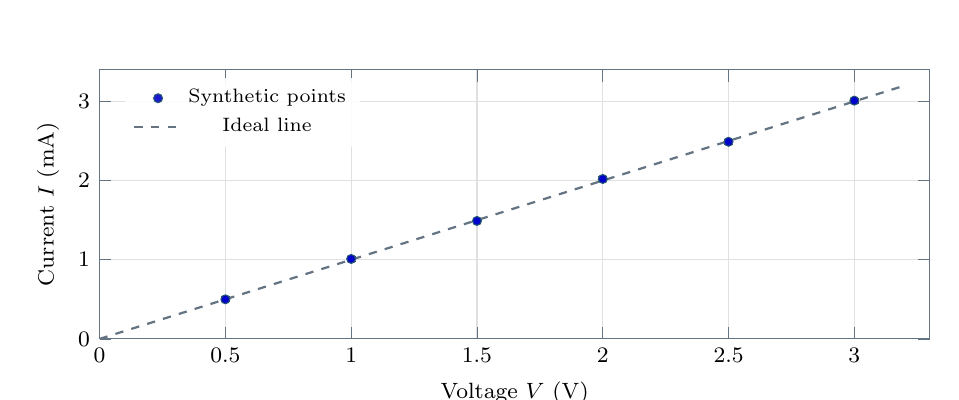
\begin{tikzpicture}
        \begin{axis}[
            width=\columnwidth,
            height=5cm,
            xlabel={Voltage \(V\) (\(\mathrm{V}\))},
            ylabel={Current \(I\) (\(\mathrm{mA}\))},
            xmin=0, xmax=3.3,
            ymin=0, ymax=3.4,
            grid=major,
            grid style={draw=reportgrid},
            axis line style={draw=reportmuted},
            tick style={draw=reportmuted},
            tick label style={font=\footnotesize},
            label style={font=\footnotesize},
            legend style={font=\scriptsize,at={(0.03,0.97)},anchor=north west,draw=none,fill=white,fill opacity=0.9,text opacity=1},
        ]
            \addplot+[only marks, mark=*,mark size=1.6pt,color=reportaccent,error bars/.cd,y dir=both,y explicit] coordinates {
                (0.50,0.50) +- (0,0.03) (1.00,1.01) +- (0,0.03) (1.50,1.49) +- (0,0.03)
                (2.00,2.02) +- (0,0.03) (2.50,2.49) +- (0,0.03) (3.00,3.01) +- (0,0.03)
            };
            \addlegendentry{Synthetic points}
            \addplot+[no marks,thick,dashed,color=reportmuted,domain=0:3.2,samples=2] {x};
            \addlegendentry{Ideal line}
        \end{axis}
    \end{tikzpicture}
    \caption{Illustrative current-voltage relationship using fictional points.}
    \label{fig:current-voltage}
\end{figure}

\section{Discussion}
\label{sec:discussion}
Interpret the results and compare them with theoretical expectations. For
example, a resistance can be calculated from a suitable current-voltage
relationship. For a ratio \(R=V/I\), a simple uncertainty expression with
independent inputs is
\begin{equation}
    \frac{u(R)}{R} \approx
    \sqrt{
       \left(\frac{u(V)}{V}\right)^2+
       \left(\frac{u(I)}{I}\right)^2
    }.
    \label{eq:uncertainty}
\end{equation}
Real data analysis also requires attention to correlated uncertainties,
instrument offsets, calibration and the appropriateness of a linear model.
In your own report, discuss limitations explicitly and avoid treating a
visually straight line as proof that all assumptions are satisfied.

\section{Conclusion}
Summarise the scientific outcome, the principal uncertainty and one realistic
improvement. Remove every fictional data point and statement before
submitting a real laboratory report.

\bibliographystyle{unsrtnat}
\bibliography{references}

% OPTIONAL FULL-WIDTH TABLE:
% Uncomment this block if you need a table that spans both columns.
% Note that table* floats to the top of a later page in standard LaTeX.
%
% \begin{table*}[t]
%   \centering
%   \caption{Synthetic values, shown here as a full-width table example.}
%   \label{tab:wide}
%   \begin{tabular}{@{}rrrrrr@{}}
%     \toprule
%     Applied voltage (\(\mathrm{V}\)) & 0.50 & 1.00 & 1.50 & 2.00 & 2.50 \\
%     \midrule
%     Current (\(\mathrm{mA}\)) & 0.50 & 1.01 & 1.49 & 2.02 & 2.49 \\
%     \bottomrule
%   \end{tabular}
% \end{table*}

\end{document}
